\section{Processor Optimizations}
\label{sec:processor_opt}

\subsection{Back-End Extensions}
Our backend extensions perform three critical functions in the optimization of DNN training code: (i) generate optimized versions of loops in the training code based on computation sparsity, (ii)  for each loop that is optimized, maintain a lookup table of the optimized versions which the frontend uses to redirect execution to optimized codes,  and (iii) maintain a code cache for storing optimized loop codes. 

\subsubsection{Generating Optimized Loop Codes}
The goal of the optimizer is to generate more efficient versions of the loops in the training code that will boost training performance when executed in place of the original loop codes.  The efficient loop versions are obtained by by applying aggressive loop optimizations that are predicated on assumptions of sparsity in loop data and computation.  Thus, the optimized loop codes can only be executed when the underlying conditions hold true. 


The goal of the optimizer is to generate efficient versions of the loops in the training code, and coordinating with the frontend to ensure that an optimized version of a loop is executed instead of the original only in the right conditions.   Our loop optimizations are predicated on the condition that an input data of the loop is zero,  and so the optimized loop version can only be executed when that condition holds.  

\begin{figure}[h]
\centering
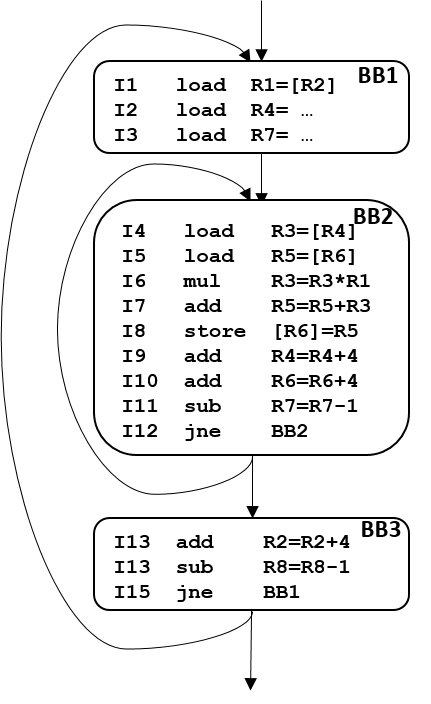
\includegraphics[height=1.8in]{Figures/weight-delta-code.png}
\caption{Code forcomputing  weight deltas (Figure~\ref{fig:deltas_source_code}).}
\label{fig:deltas_machine_code}
\end{figure}


\subsubsection{Executing Optimized Loop Codes}


\begin{figure}[h]
\centering
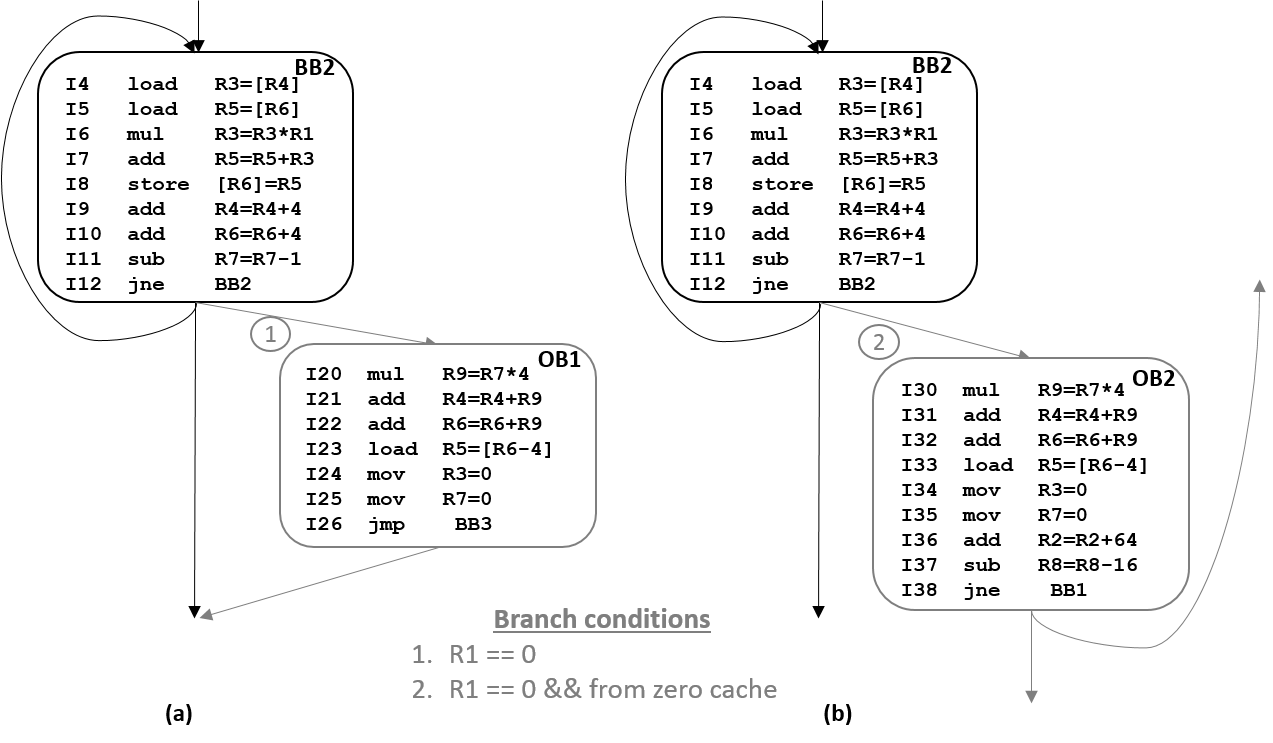
\includegraphics[height=1.8in, width=.95\columnwidth]{Figures/loop-invariant-zopt.png}
\caption{Optimizing for loop invariant zero data (R1): (a) for data from data cache, redirect execution to skip inner loop, and (b) for data from zero cache (i.e., cluster of $16$ zero data values) redirect execution to skip 16 executions of inner loop.}
\label{fig:deltas_loop_inv_opt}
\end{figure}



\begin{figure}[h]
\centering
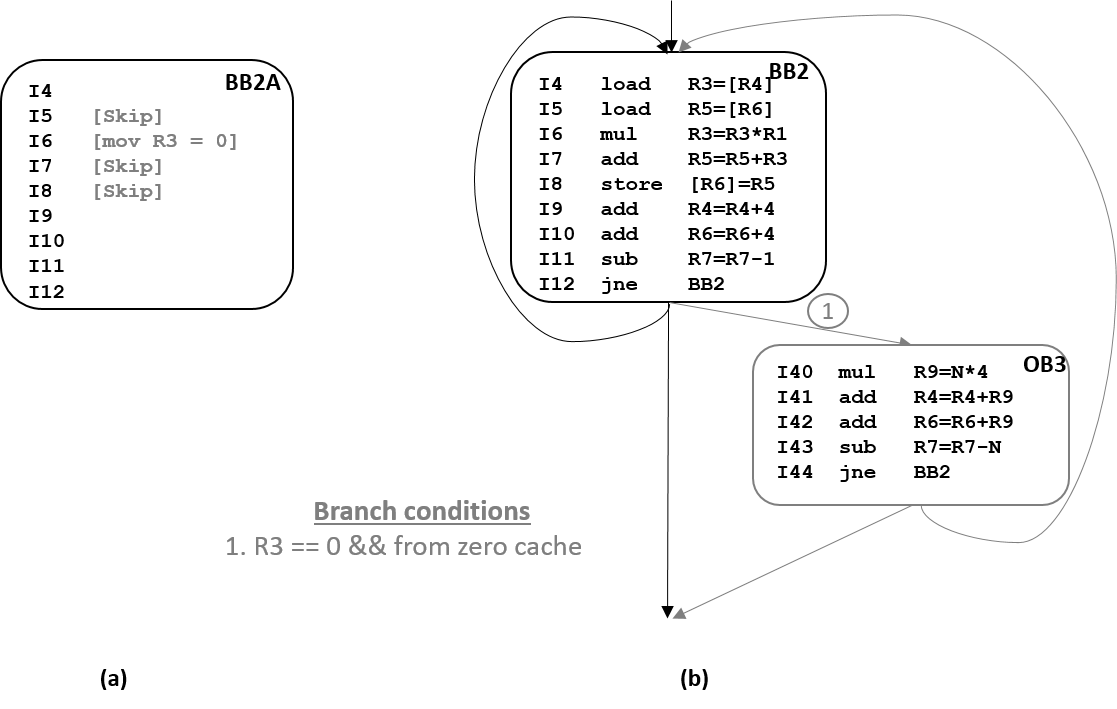
\includegraphics[height=1.8in, width=.95\columnwidth]{Figures/loop-variant-zopt.png}
\caption{Optimizing for loop variant zero data (R3):  (a) annotate code block actions to be taken by frontend, and (b) redirect execution for data from zero cache.}
\label{fig:deltas_loop_var_opt}
\end{figure}

\subsubsection{Storing Optimized Loop Codes}


\subsection{Front-End Extensions}
